\documentclass[brazil,pagestart=firstchapter]{abnt}

% This does not accept all Unicode chars (for instance: I²C gives an error)
%\usepackage[utf8]{inputenc}

% This adds support for Unicode chars.
\usepackage{ucs}
\usepackage[utf8x]{inputenc}

\usepackage[brazil]{babel}

% http://tex.stackexchange.com/questions/664/why-should-i-use-usepackaget1fontenc
% http://texblog.net/latex-archive/fonts/symbols/
\usepackage[T1]{fontenc}

% Use another font:
% http://tex.stackexchange.com/questions/553/what-packages-do-people-load-by-default-in-latex/951#951
%\usepackage{lmodern}

% 'microtype' improves LaTeX line-breaking algorithm by using
% microtypographic features of the font
% http://tex.stackexchange.com/questions/349/what-is-the-practical-difference-between-latex-and-pdflatex/358#358
\usepackage{microtype}


%%%%%%%%%%%%%%%%%%%%%%%%%%%%%%%%%%%%%%%%%%%%%%%%%%%%%%%%%%%%
% Acronyms and abbreviations

% Simple and effective acronym package:
\usepackage[printonlyused,withpage]{acronym}

% This one from abntex does not work correctly:
% http://comments.gmane.org/gmane.comp.tex.brazilian/13365
%\usepackage{tabela-simbolos}

% "nomencl" is quite annoying to use, specially when compared to "acronym".
% "nomencl" requires an external file and some extra commands.
% "acronym", on the other hand, just works out of the box!
%\usepackage{nomencl}
%\makenomenclature
% http://en.wikibooks.org/wiki/LaTeX/Indexing#Abbreviation_list
% http://franz.kollmann.in/latex/latex.html#abbr
% latexmk needs a custom dependency for this package
% http://magic.aladdin.cs.cmu.edu/2007/11/06/continuous-latex-compilation-using-latexmk/


%%%%%%%%%%%%%%%%%%%%%%%%%%%%%%%%%%%%%%%%%%%%%%%%%%%%%%%%%%%%
% Other packages

% Adding \textsubscript{}
% LaTeX already has \textsuperscript, but lacks \textsubscript.
% http://en.wikibooks.org/wiki/LaTeX/Formatting#Text_mode_superscript_and_subscript
\usepackage{fixltx2e}

% Better handling of space after a custom command.
% http://tex.stackexchange.com/questions/17730/newcommand-and-spacing
\usepackage{xspace}

% Avoid floats and figures from crossing a section boundary
% http://en.wikibooks.org/wiki/LaTeX/Floats,_Figures_and_Captions#Keeping_floats_in_their_place
\usepackage[section]{placeins}

% Required for including graphics
\usepackage{graphicx}

% SI Units
% https://bitbucket.org/josephwright/siunitx/issue/100/undefined-control-sequence-bit-and-byte
\usepackage{siunitx}
\sisetup{
	load-configurations = binary,
	per-mode = symbol,
	list-final-separator = { e },
	range-phrase = { a },
	output-decimal-marker = {,}
}

% To find the total number of pages
%\usepackage{lastpage}

%%%%%%%%%%%%%%%%%%%%%%%%%%%%%%%%%%%%%%%%%%%%%%%%%%%%%%%%%%%%
% Embedding source-code

% For inserting source-code
%\usepackage{listings}
% TODO: configure this

% Settings I had from another project:
%% Setting the default listings font size
%\lstset{
%	basicstyle=\ttfamily\footnotesize
%}
%
%% AVISO!!!
%% Dentro dos exemplos de código-fonte abaixo, coloquei um "tab" de
%% indentação por estar dentro de um "frame", e "espaços" para a
%% indentação do código de exemplo. Isto foi necessário porque os tabs
%% estavam sendo ignorados dentro do códigos de exemplo.
%
%\lstnewenvironment{shellcode}[1][]
%{\lstset{language=bash,
%	basicstyle=\ttfamily\footnotesize,
%	escapeinside={(*@}{@*)},
%	breaklines=true,
%	breakatwhitespace=true,
%	showspaces=false,
%	showstringspaces=false,
%	frame=shadowbox,
%	rulecolor=\color{black},
%	rulesepcolor=\color{black},
%	#1}
%}{}
%
%\lstnewenvironment{pythoncode}[1][]
%{\lstset{language=Python,
%	basicstyle=\ttfamily\footnotesize,
%	escapeinside={(*@}{@*)},
%	%numbers=left,
%	breaklines=true,
%	breakatwhitespace=true,
%	showspaces=false,
%	showstringspaces=false,
%	frame=shadowbox,
%	frameround=rrrt,
%	rulecolor=\color{black},
%	rulesepcolor=\color{gray},
%	#1}
%}{}


%%%%%%%%%%%%%%%%%%%%%%%%%%%%%%%%%%%%%%%%%%%%%%%%%%%%%%%%%%%%
% Table-related packages:

% For multirow cells inside tabular environments
%\usepackage{multirow}

% Longtable allows you to write tables that continue to the next page
%\usepackage{longtable}

% 'tabularx' package - simple column stretching
% http://en.wikibooks.org/wiki/LaTeX/Tables#The_tabularx_package_-_simple_column_stretching
%\usepackage{tabularx}

% 'booktabs' - Publication quality tables in LaTeX
%\usepackage{booktabs}

% Alternating row colors in tables
%\usepackage[table]{xcolor}
%\definecolor{tabular-odd-color}{gray}{0.90}
%\definecolor{tabular-even-color}{gray}{0.97}


%%%%%%%%%%%%%%%%%%%%%%%%%%%%%%%%%%%%%%%%%%%%%%%%%%%%%%%%%%%%
% Fancy headers (and footers)
% http://en.wikibooks.org/wiki/LaTeX/Page_Layout#Page_Styles
%\usepackage{fancyhdr}
%\pagestyle{fancy}
%
%% Headers and footers definition:
%\lhead{\includegraphics[height=21mm]{shared/2aliancas_h.pdf}}
%\chead{}
%% This \parbox is a hack to keep text aligned at top, but it's not the
%% only available solution:
%% http://tex.stackexchange.com/questions/2440/how-to-vertically-align-headers-footers-in-fancyhdr-package
%\rhead{\parbox[b][21mm][t]{0.65\textwidth}{\raggedleft\large\titletext \\[1em] \subtitletext}}
%\lfoot{}
%\cfoot{}
%\rfoot{Page \thepage{} of \pageref{LastPage}}
%
%\renewcommand{\headrulewidth}{0pt}  % Default is 0.4pt
%\renewcommand{\footrulewidth}{0pt}  % Default is 0pt


%%%%%%%%%%%%%%%%%%%%%%%%%%%%%%%%%%%%%%%%%%%%%%%%%%%%%%%%%%%%
% 'hyperref' for including hyperlinks to the PDF.
% It should be loaded last.
% http://en.wikibooks.org/wiki/LaTeX/Formatting#Typesetting_URLs
\usepackage{hyperref}
\hypersetup{
	pdfborder={0 0 0},
	hyperindex=false
}
% hyperindex=false is required by "tabela-de-simbolos"

% http://en.wikibooks.org/wiki/LaTeX/Labels_and_Cross-referencing#Issues_with_links_to_tables_and_figures_handled_by_hyperref
%\usepackage[all]{hypcap}


%%%%%%%%%%%%%%%%%%%%%%%%%%%%%%%%%%%%%%%%%%%%%%%%%%%%%%%%%%%%
% Custom commands

\newcommand{\VBUS}{V\textsubscript{BUS}\xspace}
\newcommand{\VDD}{V\textsubscript{DD}\xspace}
\newcommand{\GND}{GND\xspace}

%%%%%%%%%%%%%%%%%%%%%%%%%%%%%%%%%%%%%%%%%%%%%%%%%%%%%%%%%%%%
% Some metadata

% This is used only by latex-beamer package:
%\title{Mouse USB usando magnetômetro}
%\author{Denilson Figueiredo de Sá}
%\date{2011-11-16}
%\institute{DCC/UFRJ}
%\keywords{AVR, USB, mouse, magnetometer}

\autor{Denilson Figueiredo de Sá}
\titulo{Mouse USB usando magnetômetro}
\orientador{Nelson Quilula Vasconcelos}
%\comentario{}
\instituicao{Departamento de Ciência da Computação \par Instituto de Matemática \par Universidade Federal do Rio de Janeiro}
\local{Rio de Janeiro - RJ, Brasil}
\data{16 de novembro de 2011}

% latex-beamer sets the pdftitle and pdfauthor automatically, but here we
% must explicitly run it:
\hypersetup{
	pdftitle={\ABNTtitulodata},
	pdfauthor={\ABNTautordata}
}

%%%%%%%%%%%%%%%%%%%%%%%%%%%%%%%%%%%%%%%%%%%%%%%%%%%%%%%%%%%%
\begin{document}

% The "abnt" class issues a warning:
%   pdfTeX warning (ext4): destination with the same identifier
%   (name{page.i}) has been already used, duplicate ignored
% This page has a solution (or workaround):
% http://en.wikibooks.org/wiki/LaTeX/Hyperlinks#Problems_with_Links_and_Pages
%\pagenumbering{roman}
% But, anyway, it's better to ignore that warning (or even better would be
% to report it to abntex maintainers).
% Instead of messing with page numbering, I've added pagestart=firstchapter
% option.


\capa

\folhaderosto


\begin{folhadeaprovacao}

\setlength{\ABNTsignthickness}{0.4pt}
\setlength{\ABNTsignskip}{2cm}
\hspace*{1cm}

\centerline{\textbf{\large \ABNTtitulodata}}

\bigskip
\bigskip

\centerline{\textbf{\ABNTautordata}}

\bigskip
\bigskip

Projeto Final de Curso submetido ao Departamento de Ciência da Computação
do Instituto de Matemática da Universidade Federal do Rio de Janeiro como
parte dos requisitos necessários para obtenção do grau de Bacharel em
Ciência da Computação.

Apresentado por:

\assinatura{\ABNTautordata}

Aprovado por:

\assinatura{Prof. Nelson Quilula Vasconcelos \\ Orientador}
\assinatura{Prof. Adriano Joaquim}
\assinatura{Profª. Silvana Rossetto}

\bigskip
\bigskip
\bigskip

\begin{center}
\ABNTlocaldata

\ABNTdatadata
\end{center}

\end{folhadeaprovacao}


% Colocar o Sumário aqui é muito bom, mas não é de acordo com a norma ABNT
% NBR 14724: informação e documentação: trabalhos acadêmicos: apresentação.
%\tableofcontents{}


%\pretextualchapter{Dedicatória}
% TODO: escrever dedicatória (opcional)

%\pretextualchapter{Agradecimentos}
% TODO: escrever agradecimentos


\begin{resumo}
O resumo será escrito aqui.
\end{resumo}

\begin{abstract}
This will be the abstract, someday.
\end{abstract}


\listoffigures

%\listoftables


% The following command does not work:
% \listadesiglas
% Instead, I'm using "acronym" package.

\pretextualchapter{Lista de Siglas}

\begin{acronym}[EEPROM]

\acro{USB}{Universal Serial Bus}
\acro{HID}{Human Interface Device}

\acro{NRZI}{Non-Return-to-Zero Inverted}
\acro{SE0}{Single-Ended 0}
\acro{SE1}{Single-Ended 1}

\acro{I2C}[I²C]{Inter-Integrated Circuit}
\acro{TWI}{Two-Wire Interface}

\acro{SCL}{Serial Clock}
\acro{SDA}{Serial Data}

\acro{PDIP}{Plastic Dual In-line Package}
\acro{DIP}{Dual In-line Package}
\acro{QFP}{Quad Flat Package}
\acro{QFN}{Quad-Flat No-leads Package}
\acro{LCC}{Leaded Chip Carrier}

\acro{PCB}{Printed Circuit Board}

\acro{ADC}{Analog-to-Digital Converter}

\acro{ISP}{In-System Programmer}
\acro{ICSP}{In-Circuit Serial Programmer}

\acro{SRAM}{Static Random-Access Memory}
\acro{ROM}{Read-Only Memory}
\acro{EEPROM}{Electrically Erasable Programmable Read-Only Memory}

\end{acronym}


\tableofcontents


\chapter{Introdução\label{cap:introducao}}

Falar sobre: motivação, resumo, possíveis aplicações (palestras,
necessidades especiais, interatividade em jogos e exposições)

\section{Trabalhos relacionados\label{sec:trabalhos_relacionados}}

TrackIR, Wiimote, eye-tracking


\chapter{Protocolos e componentes\label{cap:protocolos_e_componentes}}

\section{USB\label{sec:usb}}

\ac{USB} é um protocolo que foi desenvolvido a partir do ano de 1994 pelas
empresas \textit{Compaq}, \textit{Hewlett-Packard}, \textit{Intel},
\textit{Lucent}, \textit{Microsoft}, \textit{NEC} e \textit{Philips}. Foi
motivado pela inexistência de um barramento bidirecional de baixo custo para
periféricos de baixa e média velocidade, assim como a falta de flexibilidade
dos barramentos até então existentes, os quais eram projetados para usos
bastante específicos, sendo impossível reutilizá-los para outros
periféricos. \cite{usb20}

A primeira versão do \ac{USB}, conhecida como ``USB 1.0'', foi oficialmente
lançada em janeiro de 1996 e definiu duas velocidades: \textit{low speed}
(\SI{1.5}{\mega\bit\per\second}) e \textit{full speed}
(\SI{12}{\mega\bit\per\second}). Alguns anos depois, em setembro de 1998, foi
lançada sua primeira revisão, ``USB 1.1'', que resolveu alguns problemas da
versão anterior mas não introduziu nenhuma mudança significativa.

A primeira grande revisão do protocolo foi lançada em abril de 2000, com o
nome de ``USB 2.0''. Esta versão introduziu uma terceira velocidade --
\textit{high speed} (\SI{480}{\mega\bit\per\second}) -- mas manteve total
compatibilidade com a revisão anterior do protocolo: dispositivos USB 1.x
funcionam em \textit{hosts} USB 2.0, e dispositivos USB 2.0 funcionam em
\textit{hosts} USB 1.x (porém limitados a \textit{full speed}).

\begin{figure}[h]
\centering
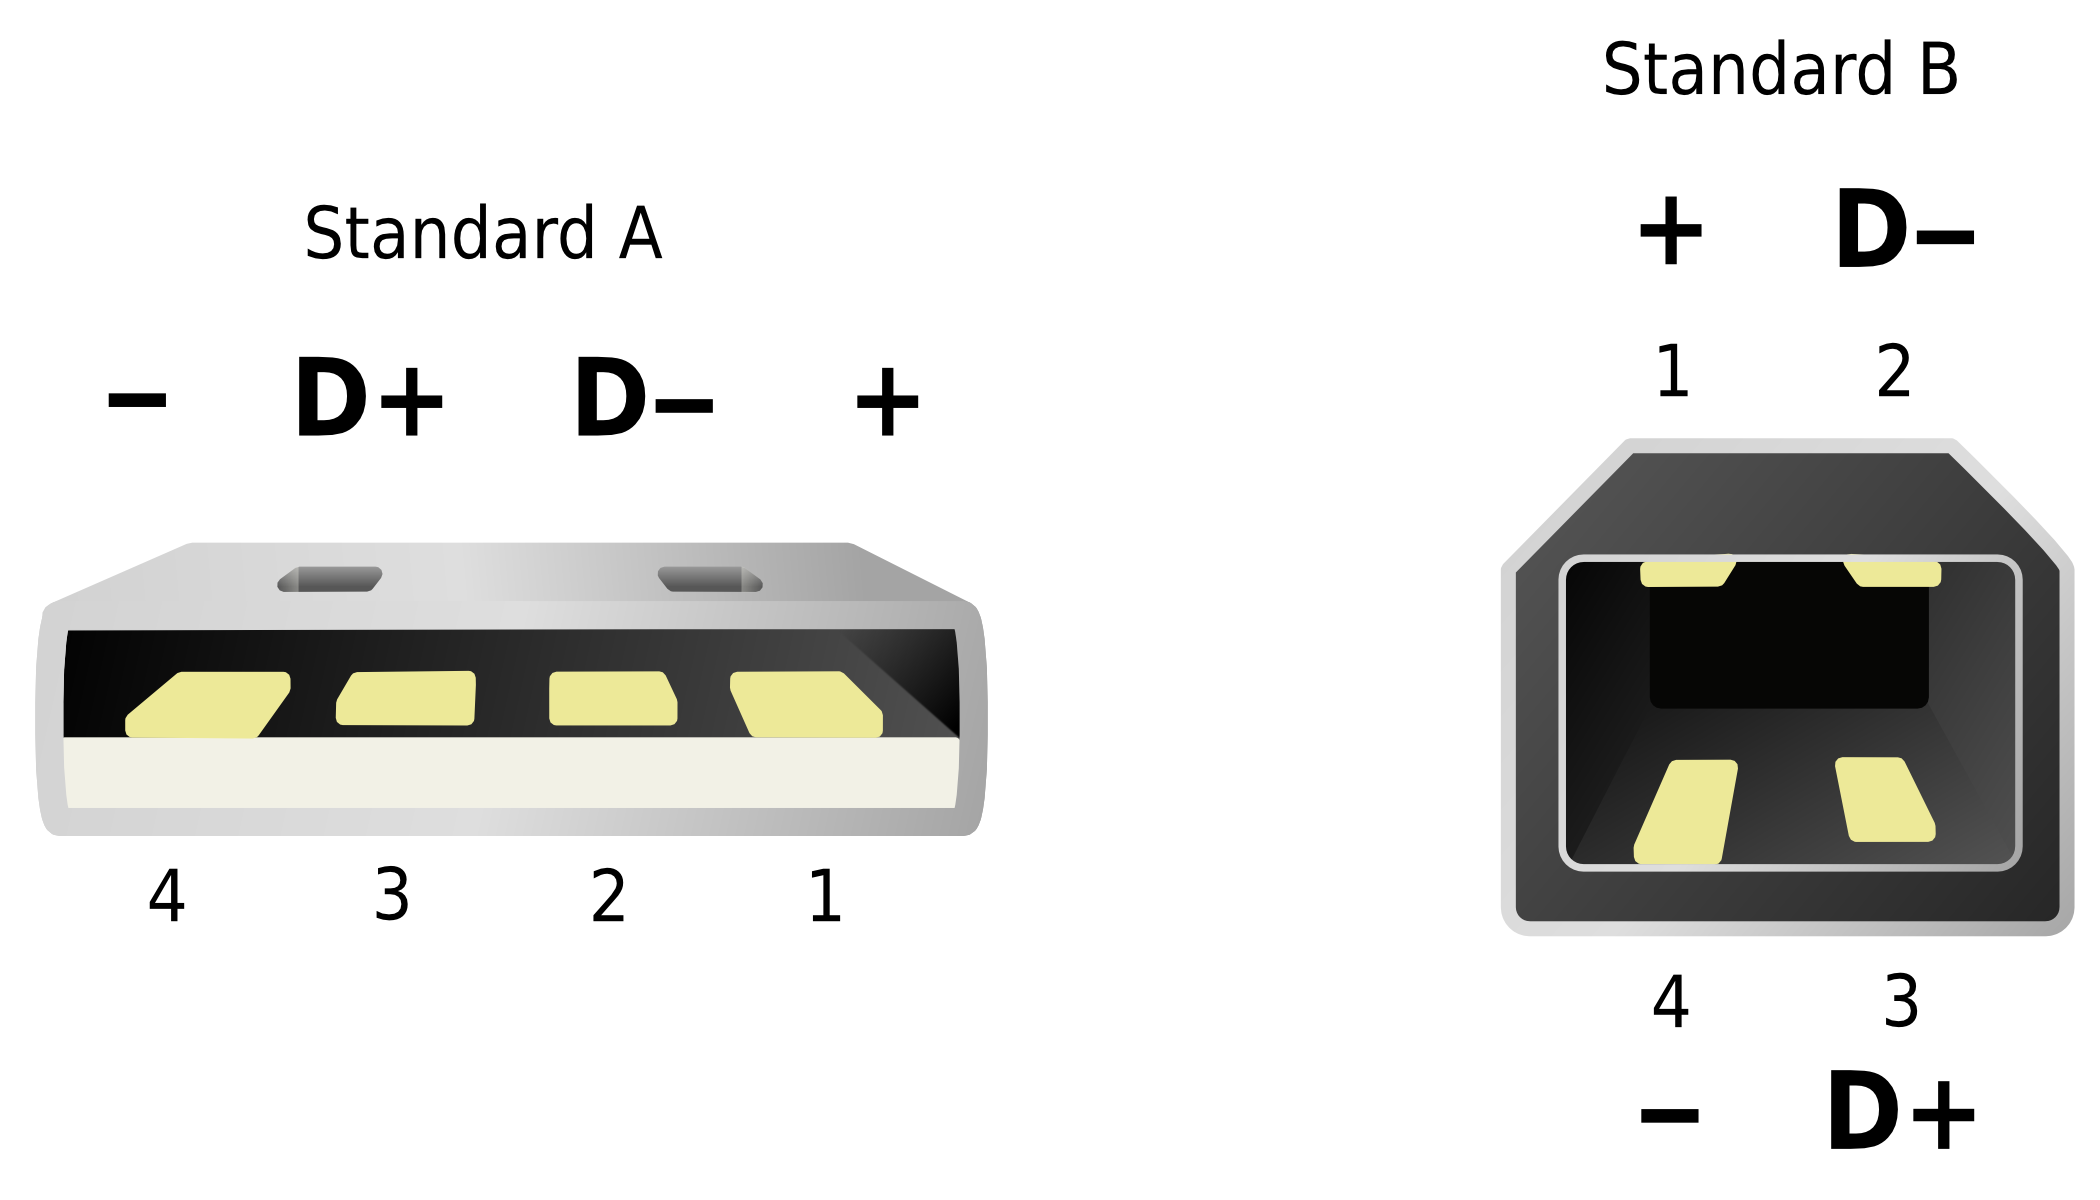
\includegraphics[width=0.5\textwidth]{img/USB.png}
\caption{Conectores do tipo A e do tipo B para USB 1.x/2.0}
\label{fig:usb_connectors}
\end{figure}

Uma conexão \ac{USB} é formada por 4 vias, sendo duas para alimentação
(\VBUS = \SI{+5}{\volt} e \GND) e duas para comunicação (D+ e D-). Os dados
são transmitidos usando a codificação \ac{NRZI} com \textit{bit stuffing}
(um ``zero'' é inserido após 6 bits ``um'' consecutivos).
\cite[p.~157]{usb20} \cite[cap.~2]{usbinanutshell}

A velocidade de um dispositivo é determinada por \textit{hardware}, de
acordo com a posição do resistor de \textit{pull-up}
	\footnote{Resistores de \textit{pull-up} ou de \textit{pull-down} servem
	para manter uma via de dados num nível lógico conhecido enquanto nenhuma
	transferência ocorre.  Normalmente possuem um valor relativamente alto
	(de \SIrange{1.5}{15}{\kilo\ohm}) para drenar pouca corrente. Um
	resistor de \textit{pull-up} conecta a via ao \VDD e a mantém no nível
	lógico 1, enquanto um resistor de \textit{pull-down} conecta a via ao
	\GND e a mantém no nível lógico 0.}
nas vias de dados. Dispositivos
\textit{low speed} possuem um resistor de \textit{pull-up} ligado ao D-,
enquanto dispositivos \textit{full speed} possuem  um resistor de
\textit{pull-up} ligado ao D+. Se não há nenhum resistor de
\textit{pull-up}, assume-se que não há nenhum dispositivo conectado.
\cite[p.~141]{usb20} \cite[cap.~2]{usbinanutshell}

Dispositivos \textit{high speed}, introduzidos no \ac{USB} 2.0, inicialmente
se identificam como \textit{full speed} (com um resistor de \textit{pull-up}
ligado ao D+), mas removem o resistor após uma negociação realizada durante
o durante o USB \textit{reset}, caso o \textit{host} também suporte
\textit{high speed}.  Caso contrário, o resistor será mantido e o
dispositivo funcionará em \textit{full speed}. Essa negociação incial
permite a compatibilidade entre dispositivos USB 2.0 \textit{high speed} e
\textit{hosts} USB 1.x. \cite[p.~142]{usb20} \cite[cap.~2]{usbinanutshell}

\begin{figure}[h]
\centering
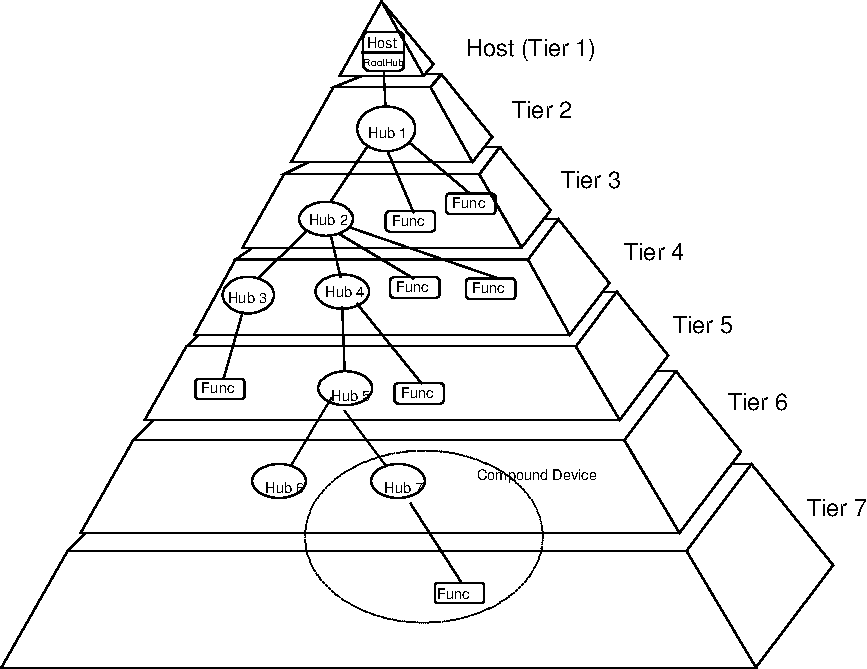
\includegraphics[width=0.75\textwidth]{img/usb_bus_topology.pdf}
\caption{Topologia do barramento USB}
\label{fig:usb_topology}
\end{figure}

A conexão de equipamentos \ac{USB} segue uma topologia de estrela em
camadas, que também pode ser entendida como uma árvore. No centro da estrela
(ou na raiz da árvore) temos obrigatoriamente o \textit{host}, que
normalmente é um computador. Por definição, o \textit{host} contém um
\textit{root hub}. Cada cabo \ac{USB} é uma conexão ponto-a-ponto que liga
um \textit{hub} da camada imediatamente acima a um dispositivo na camada
imediatamente abaixo. Um dispositivo pode ser um outro \textit{hub} ou então
uma função. Por limitações de tempo de propagação, o número máximo de
camadas é 7, incluindo a camada que contém o \textit{host}.
\cite[p.~16]{usb20}

A especificação \ac{USB} define dois tipos de conectores (conforme ilustrado
na figura \ref{fig:usb_connectors}). Um cabo \ac{USB} possui uma ponta de
cada tipo, sendo que o plugue do tipo A é conectado ao \textit{hub} da
camada acima, e o plugue do tipo B é conectado ao dispositivo da camada
abaixo. Posteriormente, foram também especificados conectores de tamanho
mais reduzido (Mini e Micro), mas os conceitos continuam os mesmos.

O protocolo de comunicação do \ac{USB} pode ser entendido como uma
arquitetura \textit{master/slave}, na qual o \textit{host} é o
\textit{master} e os dispositivos têm o papel de \textit{slave}. Só há um
\textit{host} por barramento \ac{USB}, e ele é responsável por iniciar e
gerenciar cada transação.  Como consequência, a maior parte da lógica está
centralizada no \textit{host}, simplificando bastante a implementação de
dispositivos que se conectam ao barramento \ac{USB}. \cite{usbinanutshell}

Em novembro de 2008, foi lançada a especificação do USB 3.0, que introduziu
uma quarta velocidade: \textit{super speed} (\SI{5}{\giga\bit\per\second}).
A quantidade de mudanças para suportar essa nova velocidade é grande, e foge
ao escopo deste trabalho.

% Não falei sobre:
% * Endpoints e tipos de transferências
% * *(control, interrupt, isochronous, bulk)
% * Descriptors
% * * Device Descriptor
% * * Configuration Descriptor
% * * Interface Descriptor
% * * Endpoint Descriptor
% * * String Descriptor


\section{USB HID\label{sec:usb_hid}}

De modo a permitir a existência de dispositivos \textit{plug-and-play} --
que funcionam assim que são ligados ao \textit{host}, sem necessidade de
configurações feitas pelo usuário ou de instalação de drivers específicos --
foram definidas algumas classes de dispositivos. Por exemplo, os populares
\textit{pen drives}, que substituíram os disquetes e CDs regraváveis para
transferência de arquivos, pertencem à classe \textit{USB Mass Storage}, e
os sistemas operacionais modernos já incluem suporte nativo a dispositivos
dessa classe.

Dispositivos de interface com seres humanos fazem parte da classe
\textit{USB \ac{HID}} e abrangem principalmente teclados, mouses e
joysticks. No entanto, essa classe foi projetada de forma genérica, e inclui
outros tipos de dispositivos com necessidades similares, tais como medidores
de temperatura, controles de um painel (botões, alavancas, ajustes),
volantes, pedais, leitores de códigos de barra, ou ainda novos dispositivos
que não foram previstos inicialmente na especificação. \cite[p.~1]{usbhid}

A classe \ac{USB} \ac{HID} tem como objetivos ser compacta (para reduzir o
espaço necessário no firmware do dispositivo), ser flexível e extensível,
ser genérica e auto-descritiva (de modo que cada dispositivo descreva suas
características de forma padronizada para o \textit{host}). O driver da
classe \ac{USB} \ac{HID}, presente no sistema operacional, é capaz de se
comunicar com qualquer dispositivo dessa classe. \cite[p.~2]{usbhid}

A especificação do \ac{USB} \ac{HID} foi inicialmente lançada em janeiro de
1996 (versão 1.0). Sua primeira revisão ficou disponível em abril de 1999
(versão 1.1). Sua segunda revisão, que também é a mais recente, foi lançada
em junho de 2001 (versão 1.11). Apesar desta versão ter sido lançada após o
\ac{USB} 2.0, a especificação do \ac{USB} \ac{HID} menciona apenas as duas
velocidades de dispositivos presentes no \ac{USB} 1.x, e incorretamente
chama dispositivos \textit{full speed} de \textit{high-speed}.
\cite{usbhid}


\section{I²C\label{sec:i2c}}

\ac{I2C} é um protocolo serial bidirecional desenvolvido em 1982 pela
\textit{Philips Semiconductors} (atual \textit{NXP Semiconductors}). Foi
projetado como um protocolo simples e eficiente para comunicação entre
circuitos integrados. Utiliza apenas duas vias: \ac{SCL} e \ac{SDA}.
\cite{UM10204}

A arquitetura do \ac{I2C} é baseada no modelo \textit{master/slave}, sendo
que qualquer um dos dispositivos do barramento pode assumir o papel de
\textit{master}, e inclusive o papel pode mudar ao longo do tempo. O
protocolo permite também múltiplos \textit{masters} no mesmo barramento.
\cite[p.~6]{UM10204} \cite[p.~161]{ATmega8} No entanto, para este trabalho
foi necessário apenas ligar 2 dispositivos: o microcontrolador ATmega8
(funcionando sempre como \textit{master}) e o sensor HMC5883L (funcionando
sempre como \textit{slave}).

Tanto a via de dados \ac{SDA} como a via de \textit{clock} \ac{SCL} são
bidirecionais. O \textit{master} é responsável por gerar o sinal de
\textit{clock}, mas o dispositivo \textit{slave} pode esticar o período de
\textit{clock} em determinadas situações, indicando que ainda não está
pronto para responder. \cite[p.~13]{UM10204}

A comunicação no \ac{I2C} é baseada em bytes. O \textit{master} envia um
sinal de \textit{START}, seguido de um byte de endereço. Nesse byte, 7 bits,
indicam o endereço do \textit{slave} e o oitavo bit indica o tipo de
comunicação (escrita ou leitura). Após a transmissão desse byte, o
\textit{master} libera a linha de dados e o \textit{slave} envia um bit zero
durante próximo pulso de \textit{clock}, sinalizando que recebeu o byte
(\textit{acknowledge}). \cite[p.~3]{AVR315}

Logo após o byte de endereço, inicia-se a transmissão dos bytes de dados.
Caso seja uma escrita, o \textit{master} envia os byte de dados exatamente
da mesma forma como enviou o byte de endereços, esperando pelo bit de
\textit{acknowledge} após cada byte enviado. Caso seja uma leitura, o
\textit{master} é responsável por gerar o \textit{clock} (conforme já
mencionado anteriormente), e o \textit{slave} envia um bit a cada pulso do
\textit{clock}. Após cada 8 bits recebidos (ou seja, após cada byte), o
\textit{master} deve enviar um bit de \textit{acknowledge} para o
\textit{slave}. Em outras palavras, cada byte transmitido numa direção é
sempre seguido de um bit de \textit{acknowledge} transmitido na direção
contrária. \cite[p.~3]{AVR315}

O \textit{master} finaliza uma transmissão enviando um sinal \textit{STOP},
ou então enviando um novo sinal \textit{START} para iniciar uma nova
transmissão imediatamente (condição conhecida como \textit{REPEATED START}).
\cite[p.~158]{ATmega8}

Pode-se também observar que a quantidade total de bytes transferidos é uma
escolha do \textit{master}, e o \textit{slave} não tem como saber
inicialmente quantos bytes serão requisitados.


\section{Microcontrolador ATmega8\label{sec:atmega8}}

ATmega8 é um microcontrolador de 8 bits da família AVR, fabricado pela Atmel
Corporation. Suas características principais são \cite{ATmega8}:

\begin{itemize}
\item Arquitetura Harvard, com espaços de endereçamento distintos para 
instruções e para variáveis.
\item \num{8192} bytes de memória \textit{Flash} para guardar o programa.
\item \num{512} bytes de memória \ac{EEPROM} para guardar parâmetros de
configuração do programa.
\item \num{1024} bytes de memória \ac{SRAM} volátil para as variáveis.
\item Voltagem de operação de \SIrange{4.5}{5.5}{\volt}.
\item Clock máximo de \SI{16}{\mega\hertz} usando um cristal externo.
\item Interface de comunicação serial I²C/TWI.
\item Disponível no encapsulamento PDIP
	\footnote{O encapsulamento do tipo \ac{PDIP}, também chamado de \ac{DIP},
	é o ideal para se trabalhar numa protoboard, pois o circuito integrado
	pode ser diretamente encaixado nela.}
de 28 pinos, assim como QFP e QFN
	\footnote{Para o produto final, em ambiente de produção industrial, o
	ideal é usar um encapsulamento mais compacto, como \ac{QFP} ou \ac{QFN}}
de 32 pinos.
\end{itemize}

A arquitetura dos processadores AVR foi projetada em conjunto com os
desenvolvedores do compilador de C da \textit{IAR Systems}. Como
consequência, o conjunto de instruções do AVR foi pensado de modo a
minimizar o \textit{overhead} durante a execução de programas que tenham
sido escritos em linguagens de alto nível. \cite{avr_iar_design}

Além disso, as instruções são executadas num pipeline de 2 estágios,
permitindo um desempenho máximo de 1 instrução por ciclo de \textit{clock}.
\cite[p.~9]{ATmega8} Nem sempre esse desempenho é alcançado, pois algumas
instruções (como as que acessam a memória \ac{SRAM} e os desvios) demoram
pelo menos 2 ciclos. \cite[p.~282]{ATmega8}

O microcontrolador ATmega8 inclui um módulo de comunicação serial \ac{I2C},
porém, para evitar problemas de patentes e licenças, a \textit{Atmel
Corporation} usa o nome \ac{TWI} para sua implementação dessa interface.
\cite{avrlibctwi}

Embora existam alguns modelos de microcontrolador AVR com controlador
\ac{USB} embutido \cite{atmel_avr_product_list}, o microcontrolador ATmega8
usado neste projeto não possui nenhum tipo de \textit{hardware} dedicado
para essa função. Para tal, foi usado um \textit{driver} que implementa o
protocolo \ac{USB} via software, diretamente no \textit{firmware} do
microcontrolador. Essa solução será descrita em mais detalhes na seção
\ref{sec:vusb}.


\section{Sensor HMC5883L\label{sec:sensor}}

HMC5883L é um magnetômetro fabricado pela \textit{Honeywell}. Um
magnetômetro é também conhecido como ``bússola digital'' ou ``bússola
eletrônica''.

Esse sensor trabalha de \SIrange{2.16}{3.6}{\volt} e é capaz de medir a
intensidade do campo magnético em 3 eixos perpendiculares ($X$, $Y$, $Z$)
através de um \ac{ADC} de 12 bits, chegando a uma precisão de
\SIrange{1}{2}{\degree}. Sua interface de comunicação é \ac{I2C}.
\cite{HMC5883L}

O circuito integrado possui encapsulamento \ac{LCC} e tem apenas
\num{3.0} × \num{3.0} × \SI{0.9}{\milli\metre} de tamanho. É impossível
trabalhar manualmente com algo tão minúsculo, por isso foi adquirida uma
\ac{PCB} já contendo o sensor e alguns capacitores. \cite{ebay_HMC5883L}
Essa placa possui 4 contatos, sendo metade deles para alimentação (\GND e
\VDD) e a outra metade para comunicação \ac{I2C} (SDA e SCL).

\begin{figure}[h]
\centering
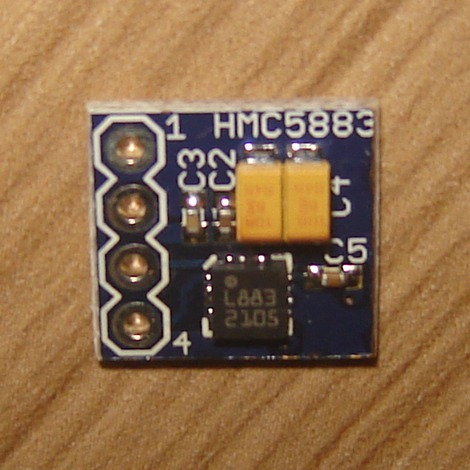
\includegraphics[width=0.45\textwidth]{img/sensor_front.jpg}
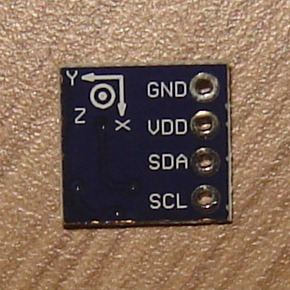
\includegraphics[width=0.45\textwidth]{img/sensor_back.jpg}
\caption{Fotos da PCB contendo o sensor}
\label{fig:sensor_photos}
\end{figure}

% TODO: falar sobre o pino DRDY (talvez falar isso só nas conclusões, ou na
% seção onde se configura o sensor


\chapter{Descrição do \textit{hardware}\label{cap:hardware}}

Explicar de maneira geral as partes do circuito.

Falar sobre microcontrolador, cristal, LEDs e botões.

Inserir aqui o diagrama do circuito.

\section{Interface USB\label{sec:hardware_usb}}

Comunicação entre a USB e o microcontrolador.

Falar sobre o resistor para indiciar low speed.

\section{Interface com o sensor\label{sec:hardware_sensor}}

Problemas com I²C. ``Fonte'' 3V3 para o sensor. Level shifting para I²C.


\chapter{Descrição do software\label{cap:software}}

\section{Bootloader\label{sec:bootloader}}

\section{Comunicação I²C/TWI\label{sec:twi}}

Falar sobre como foi implementada.

E depois falar sobre como se comunicar com o sensor (talvez em outra seção)

Internamente, o sensor possui 13 registradores que podem ser acessados pela
comunicação serial e ainda mais um registrador interno chamado de
\textit{address pointer}. Quando o \textit{master}...


\section{Driver V-USB\label{sec:vusb}}

Falar que implementa USB 1.1 (eu acho que é 1.1), low speed.
Falar sobre o consumo de 100mA.
Falar sobre os tipos de endpoints.
Falar sobre limitações, como por exemplo não
implementar o Suspend.

Falar aqui também sobre a implementação de um teclado. Talvez numa
subsection.

\section{Menu de configuração\label{sec:menu}}

Talvez falar sobre o teclado aqui dentro, não sei.

\section{Transformação de coordenadas\label{sec:coordenadas}}

Falar sobre: ferramentas auxiliares, teoria, resultados.

Falar sobre calibração dos cantos.

Falar sobre calibração do zero (ou deixar para falar isso depois).

\section{Mouse USB\label{sec:mouse}}

Falar sobre a implementação do mouse (que na verdade é absolute pointing
device).

Talvez aqui, talvez numa outra (sub)seção, falar sobre o fluxo da main().

\section{Outros problemas\label{sec:outros_problemas}}

\subsection{Debouncing dos botões\label{sec:debouncing}}

\subsection{Tamanho do firmware\label{sec:firmware_size}}

\subsection{Gravar configurações na EEPROM\label{sec:eeprom}}

Falar sobre gravar na EEPROM de maneira não bloqueante.

\chapter{Conclusões\label{cap:conclusoes}}

Resultados alcançados. O que deu certo. O que não deu certo.

\section{Trabalhos futuros\label{sec:trabalhos_futuros}}

Listar o que pode ser feito a partir deste projeto.


%%fakesection  Bibliografia

\bibliographystyle{abnt-num}
\bibliography{mouse_magnetometro_monografia}

% How to add \url{} to "url=" entries from Pybliographic:
% :%s/\(url\s*=\s*{\)\([^\\].*[^}]\)\(},\?\)/\1\\url{\2}\3/

%%fakesection  Anexo
\anexo

\end{document}

% vim:filetype=tex ts=4 sw=4 noet tw=76
